\documentclass{article} 
\usepackage{color}
\usepackage{algorithmic}
\usepackage[small,bf]{caption}
\usepackage{float}
\usepackage{graphicx}

\graphicspath{{../}}

\floatstyle{plain}
\newfloat{program}{thp}{lop}
\floatname{program}{code}


\begin{document}
    
\title{Stock Exchange Server Simulator}
\author{Anton Morozov and Shubham Chopra}
\maketitle
    
\section{Introduction}

Our goal is to create a unified format for specifying simulations from historical data. In many instances it is hard, expensive or downright impossible to create a scenario similar to the one that produced the original historic data. Usually the simulations of such scenarios are created. In simulations the data from the original experiment is augmented with new data to create variations of the original scenario. A set of user defined rules specify how the historical and the new data interact to produce the desired outcome. Below we describe a format that allows us to specify those rules freely. 

%In these simulations parameters during the progress of an experiment are preserved and we want to either change or augment those parameters with new information. Also we want to let users specify the results of the augmentation. 

\section{Approach}

At a high level, historical data together with new data can be thought of as a stream of updates to a relational table. We assume that there are $N$ update streams, each can be represented by its own relational table. These streams can be further combined or subdivided into a set of $K$ additional streams. For each $k$ in $K$ we can describe the desired simulation outcomes. The resultant output streams can then be combined, filtered and output as desired.


%parameters for the experiments can be though of as a stream of updates to a relational table.  New data can be thought of as updates to some relation. If we have $N$ update streams, we will end up with $N$ different relations. These relations can be combined into a set of $K$ additional relations. For each $k$ in $K$ we can describe desired simulation outcomes. The resultant $K$ streams can then be combined and filtered and outputted as desired. 

In this paper we will be using a stock exchange simulator as an example. The goal of the simulator is to approximate an outcome of adding buy/sell stock request to a real stock exchange. The stock exchange simulator can be thought of as a stream processor. We can assume that there are $N$ streams coming in. Each of these streams is filtered according to certain conditions and merged together if needed. The merged streams form $K$ order-books. Matching rules are applied to these $K$ order-books. These generates a set of output streams.

Generalized specification process for creating a simulator can be described in five steps:

\begin{enumerate}
    \item {\bf Input Filter}: Each input stream can be filtered. This means that each incoming tuple in the stream can either be removed or it can generate extra inputs. 
    \item {\bf Input Merging}: The set of input streams can be combined or subdivided into another set of $K$ streams using merging and filtering. 
    \item {\bf Simulator Rules Application}: Each set of streams produced at a merging stage is materialized as a set of relations. These relations are reduced/matched using rules given by a user.
    \item {\bf Output Merging}: Experiment outcome streams can again be combined or filtered.
    \item {\bf Output Filter}: For each output stream additional conditions can be imposed. Data within a stream can be changed based on those conditions.
\end{enumerate}

\begin{figure}
  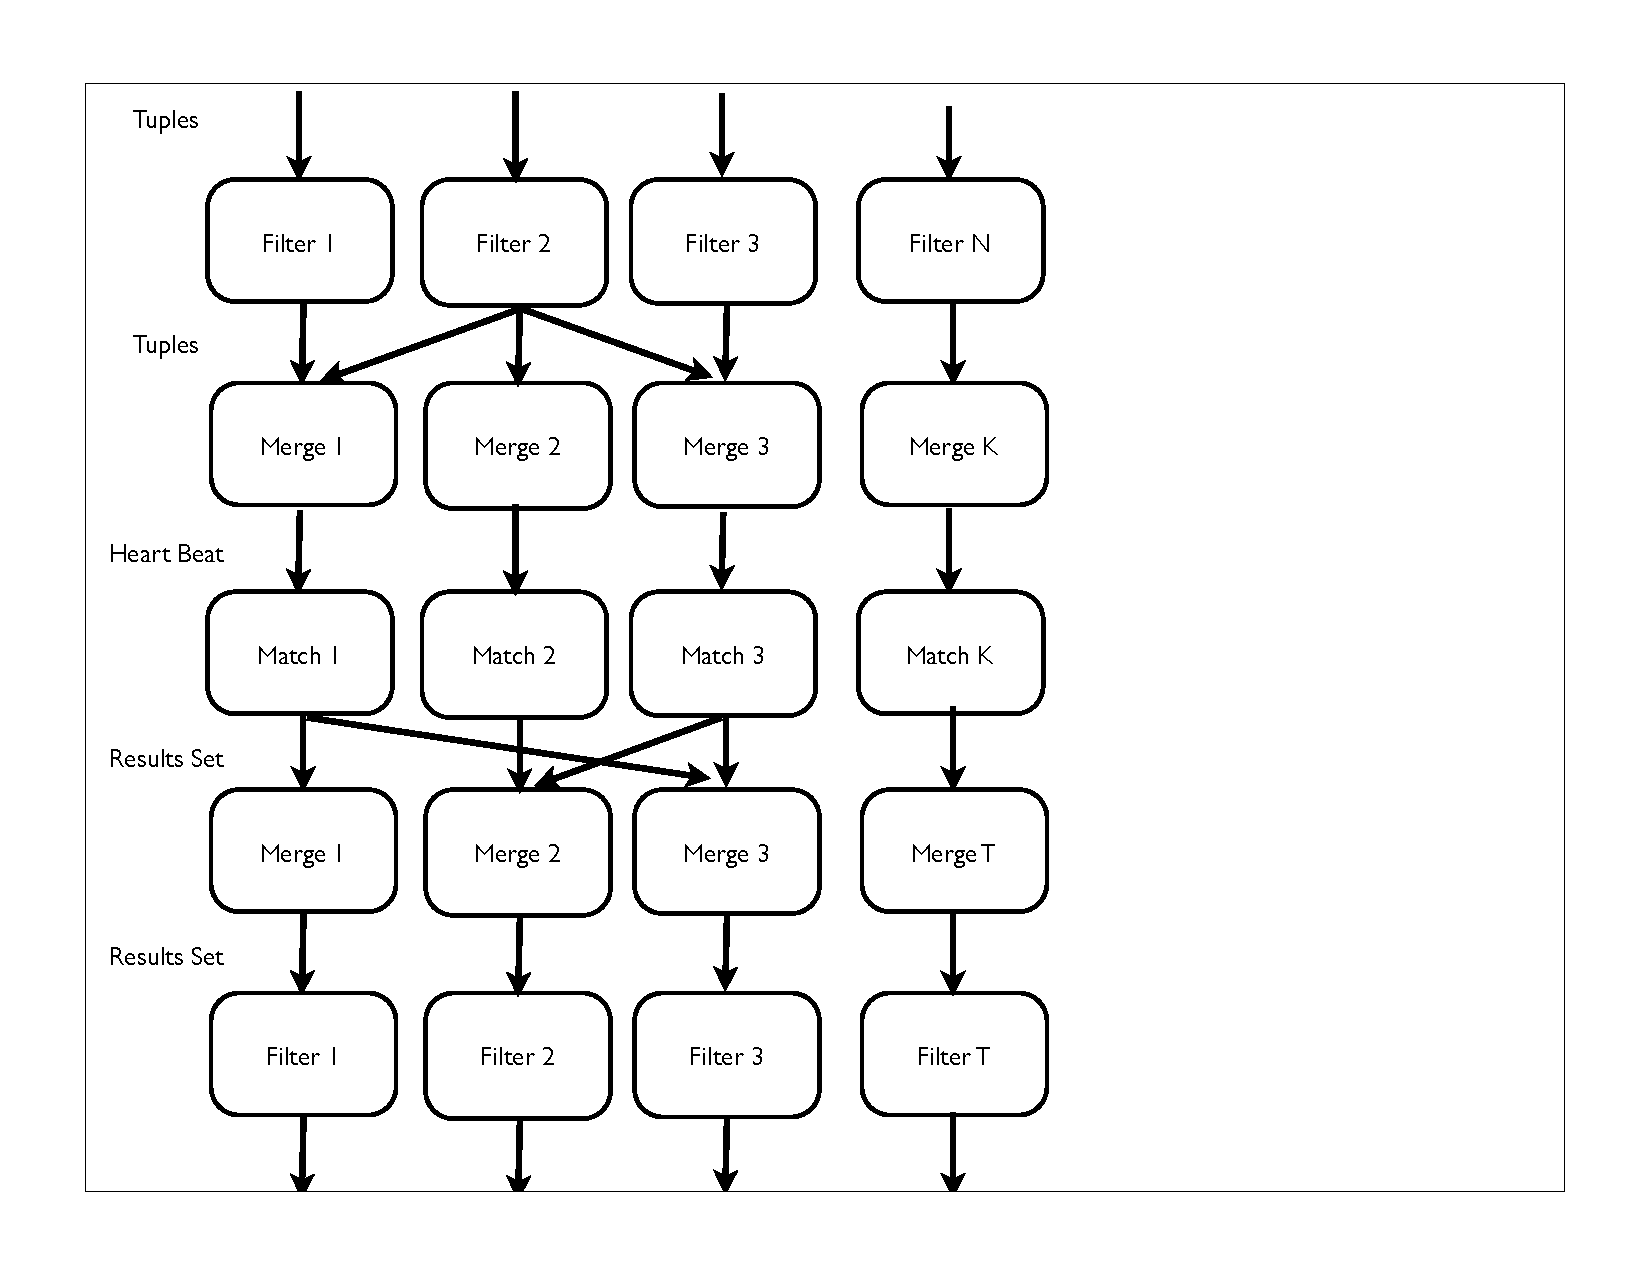
\includegraphics[width=4.50in]{figures/ExchangeFigure.pdf}
  \caption{Exchange Execution Path.}
  \label{fig:overview}
\end{figure}

Figure \ref{fig:overview} shows data execution paths and interactions between various components of the Exchange Server.

\section{Running Example}

The Exchange Server Simulator is going to be our example throughout this presentation. In particular we will show how one specific matching strategy can be implemented using this framework.

The Exchange Server Simulator uses historical data from previously occurred "real" stock exchanges to predict the outcomes of adding buy/sell stock orders from a novel strategy. This evaluates a trading strategy. The buy/sell orders from a new new strategy are combined with "real" trades using the following way. If a strategy's order can be matched with some historic order a new order equal to historic order is added to the mix, otherwise a historic order are matched with a historic order and an order from a trading strategy is matched with another order from a trading strategy.

\section{Input Filter}

An input filter is a \emph{stream-to-stream} transformation. It is used to remove undesired updates from input stream or to add them to the stream triggered by some input parameters.

The desired functionality for a filter is as follows:

\begin{itemize}
    \item Get an input tuple
    \item Check if a tuple satisfies conditions
    \item If conditions are met, forward tuple to another stream
    \item If conditions are not met, discard the tuple
\end{itemize}

The functionality for an insertion trigger.

\begin{itemize}
    \item Get an input tuple
    \item Check if a tuple satisfies trigger conditions
    \item If conditions are met, create a tuple and forward it a desired stream
    \item If conditions are not met, ignore
\end{itemize}


\noindent SQL can be used to filter incoming tuples. For instance the code to filter out tuples will look like:

\begin{verbatim}   
    SELECT * as new_stream
    FROM input_stream
    WHERE tuple_condition
\end{verbatim}

\noindent Similarly extra tuples can be added with SQL based on some trigger conditions,

\begin{verbatim}   
    INSERT INTO new_stream new_tuple(tuple)
    SELECT tuple
    FROM input_stream
    WHERE trigger_condition
\end{verbatim}

\noindent where a {\tt new\_tuple(tuple)} statement is a shorthand for a creation of new tuple based on a tuple from input stream.

In our example the Exchange Server has two input streams. One stream is historical data from trades executed at some previous date. The second stream is additional trades coming from Trading Algorithms. The stream of updates coming from Trading Algorithms can be controlled by the user (at the moment we assume that users have complete control over trading algorithms). However, historical data can be dirty and incomplete. We want to give users control to restore or remove information impurities. For instance, data tuples, corresponding to orders that were completed, can be removed from the system since the Simulator will be able to create such a matching by itself. Also if we see a change in some order (the order was partially fulfilled) and we have no reference to such order in the order book, we would want to add such an order to the book (the concerns for this operation are noted later).

Exchange Server Filtering can be implemented in the following way:

From the above the two input streams  are a \emph{historic\_input\_stream} stream and a \emph{simulated\_input\_stream} stream. We create filters to remove undesired tuples:

\begin{verbatim}   
    SELECT * 
    FROM historic_input_stream HS
    WHERE HS.action=='B' &&
          HS.action=='S' &&
          HS.action=='D'
    INTO HFS
\end{verbatim}

\begin{verbatim}  
    SELECT *
    FROM simulated_input_stream SS
    WHERE SS.action=='B' &&
          SS.action=='S' &&
          SS.action=='D'
    INTO SFS
\end{verbatim}

\noindent We also need to forward these data to output streams,

\begin{verbatim}   
    SELECT * 
    FROM historic_input_stream HS
    WHERE HS.action=='B' &&
          HS.action=='S' &&
          HS.action=='D'
    INTO output_stream
\end{verbatim}

\begin{verbatim}  
    SELECT *
    FROM simulated_input_stream SS
    WHERE SS.action=='B' &&
          SS.action=='S' &&
          SS.action=='D'
    INTO output_stream
\end{verbatim}

\noindent where an \emph{output\_stream} stream is an only output of the simulator. 


\section{Input Merging}

Often, once input is received, we would want to combine (join/union) two input streams or to impose future conditions (example windowing) on the input steam. Input Merging is also a \emph{stream-to-stream} transformation.

%, which will allow users to specify those conditions and creates additional relations from them.

The desired functionality is simple.
\begin{itemize}
    \item Get tuple from a set of input streams
    \item Forward tuple to output stream
\end{itemize}


\noindent In SQL we can combine two input streams if they have the same schema 

\begin{verbatim}   
    input_stream1
    UNION
    input_stream2
    UNION
    ...
    INTO output_stream
\end{verbatim}


A set of streams produced as a result of merging are matched in the Exchange Server. Merging provides a way to combine streams over which matching will be imposed. 

The Exchange Server uses merging to duplicate historical data and merge it with the updates from new strategies.

\begin{verbatim}  
    HFS
    UNION
    SFS
    INTO combinedView
\end{verbatim}

A \emph{combinedView} stream will contain tuples from the historic data stream and the algorithm's produced stream. 

In many cases we will want to distinguish between tuples coming from different streams

\begin{verbatim}  
    (SELECT augmented_tuple_historic
     FROM HFS hs)
    UNION
    (SELECT augmented_tuple_simulated
     FROM SFS ss)
    INTO combinedView
\end{verbatim}

Here constructs \emph{augmented\_tuple\_historic} and \emph{augmented\_tuple\_simulated} are a short for:

\begin{verbatim}
    augmented_tuple_historic -> hs.id, hs.time, hs.action,
                            hs.volume, hs.price, source="hist"
    augmented_tuple_simulated -> ss.id, ss.time, ss.action,
                            ss.volume, ss.price, source="sim"
\end{verbatim}

The above merging allows us to expand a tuple's schema, to include the tuples source. 

\begin{verbatim} 
    HFS INTO historicView
\end{verbatim}

From above merging produces two streams: \emph{combinedView} and\emph{historicView}. A \emph{historicView} stream contains filtered tuple only from a \emph{HFS} stream. A \emph{combinedView} stream contains tuples from both a \emph{HFS} and a \emph{SFS} streams. The \emph{combinedView} stream's schema can be expand if needed.


\section{Simulator Rules}

Simulator rules are a set of user definitions on how to create relations from input streams. They show how to reduce those relations and to produce an output stream of events. 

\subsection{Stream to Relations}
All actions performed so far were \emph{stream-to-stream} actions. These actions allowed us to manipulate streams of incoming data to create a stream of updates to a set of relations. We need to materialize the streams into a set of relations to apply user defined rules to them. 

In our running example we would want to visualize the bid and the ask order books into two relations. Each stream produced at an Input Merging stage will have a bid and an ask books.

The bids order book is visualized as a set of buy requests over unbounded time frame.

\begin{verbatim}  
    SELECT * as bids_historicView
    FROM historicView hv
    RANGE UNBOUNDED
    WHERE hv.action=='B'
\end{verbatim}

\noindent Similarly for an asks relation.

\begin{verbatim}  
    SELECT * as asks_historicView
    FROM historicView hv
    RANGE UNBOUNDED
    WHERE hv.action=='S'
\end{verbatim}

\noindent The bid and the asks relations for the \emph{compbineView} stream are done similarly.

\begin{verbatim}  
    SELECT * as bids_combinedView
    FROM combinedView cv
    RANGE UNBOUNDED
    WHERE cv.action=='B'
\end{verbatim}

\noindent And the asks relation

\begin{verbatim}  
    SELECT * as asks_combinedView
    FROM combinedView cv
    RANGE UNBOUNDED
    WHERE cv.action=='S'
\end{verbatim}

\noindent The asks and bids relations are updated with new tuples from the stream. The stream also contains user requests to remove some tuples from those relations. This is can be accomplished with the following deletes.

\begin{verbatim}  
    DELETE *
    FROM asks_historicView av
    WHERE av.id = hv.id
            (SELECT * 
             FROM historicView
             RANGE NOW
             WHERE historicView.action='D') as hv  

    DELETE *
    FROM bids_historicView bv
    WHERE bv.id = hv.id
            (SELECT * 
             FROM historicView
             RANGE NOW
             WHERE historicView.action='D') as hv 
\end{verbatim}

Similarly we can create update order-book relations for the \emph{combinedView} stream.

\begin{verbatim}  
    DELETE *
    FROM asks_combinedView av
    WHERE av.id = cv.id
            (SELECT * 
             FROM combinedView
             RANGE NOW
             WHERE combinedView.action='D') as cv  

    DELETE *
    FROM bids_combinedView bv
    WHERE bv.id = cv.id
            (SELECT * 
             FROM combinedView
             RANGE NOW
             WHERE combinedView.action='D') as cv 
\end{verbatim}


\subsection{Rule Application}

The main component of our system is its ability to apply a set of user defined rules. This provides users with a ability to manipulate the relations. The rules define how the output stream for a group of relations is produced and how the existent relations are changed. 

\begin{verbatim}
    REDUCE_LOOP [WHILE condition | TIMES number]
    FROM [NEW] relation1, [NEW] relation2, ... 
    WHEN condition1
        (set of statements to be executed)
    WHEN condition2
        ...
    WITH HEARTBEAT ON (tuple identifier)
    EVERY [number TUPLE | time INTERVAL] IN relation 
\end{verbatim}

The {\tt REDUCE\_LOOP} statement gives users a possibility to show with a simple set of statements what are the consequences of some events. The statement provides an ability to execute a set of actions when a condition is satisfied. The conditions are specified by the {\tt WHEN} clause followed by a set of SQL statements to be executed in case the condition is true. The conditional statements can be executed repeatedly when conditions {\tt WHILE} or {\tt TIMES} are present. A {\tt WHILE} predicate followed by a condition indicates that the statements should be executed until the condition is true. A {\tt TIMES} predicate indicates how many times the conditions should be executed. A {\tt FROM} predicate indicates what tables the data is coming from, on which the {\tt WHILE} condition is applied. A field specifier {\tt NEW} indicates that the content of the table should be updated. The need to update can come as a result of new tuples inserted into a relation from an input stream or as a consequence of the executed statements.   

In our running example of the Exchange Server, we provide rules where if the price on the best ask order and best bid order match we remove/update them from/in the tables and send consequences of the update to the output stream.

Before we start matching we need to define relations we will be using later.

\begin{verbatim}      
    SELECT * as min_bid_price
    FROM bids_historicView bhv
    WHERE bhv.price = (SELECT min(price) FROM  bids_historicView))
    
    SELECT * as top_bid
    FROM min_bid_price mbp
    WHERE mbp.time = (SELECT min(time) FROM min_bid_price)
    
    SELECT * as max_ask_price
    FROM asks_historicView ahv
    WHERE ahv.price = (SELECT max(price) FROM  asks_historicView))
    
    SELECT * as top_ask
    FROM max_ask_price map
    WHERE map.time = (SELECT min(time) FROM max_ask_price)
\end{verbatim}

We can start matching using above specification.

\begin{verbatim}  
    REDUCE_LOOP WHILE top_bid.price<=top_ask.price
    FROM NEW top_bid, NEW top_ask
    WHEN top_bid.volume = top_ask.volume 
            (DELETE * FROM bids_historicView bhv 
                      WHERE bhv.id = top_bid.id,
             DELETE * FROM asks_historicView ahv 
                      WHERE ahv.id = top_ask.id,
             INSERT INTO historic_output: 
                        create_F(top_bid), create_F(top_ask))
    WHEN top_bid.volume < top_ask.volume 
            (DELETE * FROM bids_historicView bhv 
                      WHERE bhv.id = top_bid.id,
             INSERT INTO asks_historicView: create_E(top_ask) 
                ON DUPLICATE KEY UPDATE id = top_ask.id
             INSERT INTO historic_output:
                        create_F(top_bid), create_E(top_bid))
    WHEN top_bid.volume > top_ask.volume 
            (DELETE * FROM asks_historicView ahv 
                      WHERE ahv.id = top_ask.id,
             INSERT INTO bids_historicView: create_E(top_bid) 
                 ON DUPLICATE KEY UPDATE id = top_bid.id
             INSERT INTO historic_output:
                        create_F(top_ask), create_E(top_bid))
    WITH HEARTBEAT ON *
    EVERY 1 TUPLE IN historicView
\end{verbatim}

In the above we compute tables {\tt top\_bid} and {\tt top\_ask} containing the best ask tuple and the best bid tuple on every iteration. We continue to iterate through the loop until the top bid and the top ask tuples cannot be matched on price. Depending on the amount of stocks in the bid and ask order the consequences of matching are also different. This matching rule is initiated on every update tuple to the \emph{historicView} stream. 

We need to define helper relations, before starting matching

\begin{verbatim}      
    SELECT * as min_bid_price
    FROM bids_combinedView bhv
    WHERE bhv.price = (SELECT min(price) FROM  bids_historicView))
    
    SELECT * as top_bid
    FROM min_bid_price mbp
    WHERE mbp.time = (SELECT min(time) FROM min_bid_price)
    
    SELECT * as max_ask_price
    FROM asks_combinedView ahv
    WHERE ahv.price = (SELECT max(price) FROM  asks_historicView))
    
    SELECT * as top_ask
    FROM max_ask_price map
    WHERE map.time = (SELECT min(time) FROM max_ask_price)
\end{verbatim}

The {\tt REDUCE\_LOOP} statement for the \emph{combinedView} stream is very similar to the above. 

\begin{verbatim}  
    REDUCE_LOOP WHILE top_bid.price<=top_ask.price
    FROM NEW top_bid, NEW top_ask
    WHEN top_bid.volume = top_ask.volume 
            (DELETE * FROM bids_combinedView bcv 
                      WHERE bcv.id = top_bid.id,
             DELETE * FROM asks_combinedView acv 
                      WHERE acv.id = top_ask.id,
             INSERT INTO combined_output:
                      SELECT create_B(top_bid)
                      FROM top_bid t
                      WHERE t.source="hist" && top_ask.source="sim"
             INSERT INTO combined_output:
                      SELECT create_S(top_ask)
                      FROM top_ask t
                      WHERE t.source="hist" && top_bid.source="sim"
             INSERT INTO combined_output: 
                      SELECT create_F(top_bid), create_F(top_ask)
                      FROM top_bids b, top_ask a
                      WHERE not(b.source="hist" && a.source="hist"))
    WHEN top_bid.volume < top_ask.volume 
            (DELETE * FROM bids_combinedView bcv 
                      WHERE bcv.id = top_bid.id,
             INSERT INTO asks_combinedView: create_E(top_ask) 
                ON DUPLICATE KEY UPDATE id = top_ask.id
             INSERT INTO combined_output:
                      SELECT create_B(top_bid)
                      FROM top_bid t
                      WHERE t.source="hist" && top_ask.source="sim"
             INSERT INTO combined_output:
                      SELECT create_S(top_ask)
                      FROM top_ask t
                      WHERE t.source="hist" && top_bid.source="sim"
             INSERT INTO combined_output: 
                      SELECT create_F(top_bid), create_F(top_ask)
                      FROM top_bids b, top_ask a
                      WHERE not(b.source="hist" && a.source="hist"))
    WHEN top_bid.volume > top_ask.volume 
            (DELETE * FROM asks_combinedView acv 
                      WHERE acv.id = top_ask.id,
             INSERT INTO bids_combinedView: create_E(top_bid) 
                 ON DUPLICATE KEY UPDATE id = top_bid.id
             INSERT INTO combined_output:
                     SELECT create_B(top_bid)
                     FROM top_bid t
                     WHERE t.source="hist" && top_ask.source="sim"
             INSERT INTO combined_output:
                     SELECT create_S(top_ask)
                     FROM top_ask t
                     WHERE t.source="hist" && top_bid.source="sim"
             INSERT INTO combined_output: 
                     SELECT create_F(top_bid), create_F(top_ask)
                     FROM top_bids b, top_ask a
                     WHERE not(b.source="hist" && a.source="hist"))
    WITH HEARTBEAT ON *
    EVERY 1 TUPLE IN combinedView
\end{verbatim}

The matching rule for the \emph{combinedView} stream is more complicated than the matching rule for the \emph{historicView} stream. This is caused by the need to insert a duplicate of a matched historic tuple into an output stream.

\subsection{REDUCE\_LOOP Simplifications}

It is possible to simplify the functionality of a {\tt REDUCE\_LOOP} statement by removing a {\tt HEARTBEAT} condition out of it. The purpose of the {\tt HEARTBEAT} is to indicate when the {\tt REDUCE\_LOOP} statement should be executed. 

The {\tt HEARTBEAT} condition is tied up with some stream. This means we can remove it from the definition of the {\tt REDUCE\_LOOP} statement and create a stand alone statement for some stream. 

\begin{verbatim}
    APPLY HEARTBEAT TO reduce_loop_name1, reduce_loop_name2, ...
    ON stream
    EVERY [number TUPLE | time INTERVAL] IN relation
\end{verbatim}

This condition imposed to a stream will trigger {\tt REDUCE\_LOOP} statements by the given names. 

Consequently a {\tt REDUCE\_LOOP} statement will be modified as follows.

\begin{verbatim}
    REDUCE_LOOP name [WHILE condition | TIMES number]
    FROM [NEW] relation1, [NEW] relation2, ... 
    WHEN condition1
        (set of statements to be executed)
    WHEN condition2
        ...
\end{verbatim}

\section{Output Merging}

Output Merging is similar to Input Merging. The idea is to take streams produced by user's rules and combine them into desirable output streams. This is done similarly to Input Merging with either joining two streams on a set of attributes or doing a union of two streams.

\begin{verbatim}   
    input_stream1
    UNION
    input_stream2
    UNION
    ...
    INTO output_stream
\end{verbatim}

The Exchange Server outputs only one stream of updates. Thus, when matching occurs over a set of relations, they are combined into a single stream,  

\begin{verbatim}
    historic_output
    UNION
    (SELECT filtered_tuple
    FROM combined_output co)
    INTO output_stream
\end{verbatim}

\noindent where a stream \emph{combined\_output} is an output stream resulting from applying matching rules similar to the above to \emph{combinedView}. A stream \emph{historic\_output} is a stream resulting from the above matching rule. We cannot just combine two output streams, because they have different schemas. A \emph{combined\_output} stream has an extra field called \emph{source}, which needs to be removed first. A \emph{filtered\_tuple} parameter indicates a tuple from the \emph{combined\_output} stream without that field.

%\emph{example?}

\section{Output Filtering} 

An Output filter is the last change for a system to add changes to outgoing data. In some ways it is very similar to the input filter. It can add or project away fields in the stream. It can additionally add user defined functions to the tuples in the stream.

\begin{verbatim}
    APPLY user_function(*)
    FROM input_stream
    TO   output_stream 
\end{verbatim}

This functionality allows for users to take a tuple from the stream and change some of its parameters.

To give an example of this functionality we will look at our running example. We know from experience that stock prices respond to high volume trades by the increase in their sale price. The users can create a filter to emulate this. For example, when there is a high volume stock movement in the \emph{combined\_output} stream users might want to increase price field value in all stock transactions by a small amount for a given time frame. Thus we can add the following filter

\begin{verbatim}
    APPLY price_change(*)
    FROM output_stream
    TO   final_output 
\end{verbatim}

Here a \emph{price\_change(*)} function is defined on the output tuple. The output of the function is a changed tuple, where parameters are changed. In this case the \emph{price} field is dynamically changed. 

The function in the {\tt APPLY} statement can be dynamic depending on the triggers from various streams. It is possible to add trigers that will change internal parameters of the function to any stream in the system. In this case we might have a trigger, 

\begin{verbatim}
    SELECT *
    FROM combined_output co
    WHERE co.action="B" && co.volume>1000
\end{verbatim}

that indicated then to increase the price. 

\section{Alternative Simulator Structure}

The current structure of the Simulator creates a fair amount of data duplication. This leads to a some amount of work duplication. For example, in our example of the Exchange Simulator we have two similar reduce loops. The reduce loop, which is responsible for handling data coming from the \emph{combinedView} stream, repeats a lot of matches between historic tuples. Those matches are ignored by the reduce loop, since they are duplicated in the first reduce loop. 

Here we will present an alternative approach to the system design that reduces the amount of duplication work. The down side of this approach is a more complicated schema of the internal streams. Additionally the matching rules will have to be more complicated.  

\subsection{Input Filtering}

The input filtering component remains the same. The purpose of the filter is to remove tuples users do not care about. This need does not change with this approach. 

\subsection{Input Merging}

Previous approach used this step to duplicate the data into the various streams. This approach will merge the streams to limit the amount of duplication. The semantics of the step will remain the same but the implications will differ. In this step all the streams will be merged if they need to be used in the later reduce step.


In the example of the exchange simulator we will have. 
\begin{verbatim}
    (SELECT augmented_tuple_historic
     FROM HFS hs)
    UNION
    (SELECT augmented_tuple_simulated
     FROM SFS ss)
    INTO combinedView 
\end{verbatim}

The side effect not duplicating data is the change and unification of schemas of each input stream. 

Here \emph{augmented\_tuple\_historic} and \emph{augmented\_tuple\_simulated} constructs are a short hand for:

\begin{verbatim}
    augmented_tuple_historic -> hs.id, hs.time, hs.action,
                            hs.volume, hs.price, source="hist",
                            base_volume=hs.volume, current_volume=0
    augmented_tuple_simulated -> ss.id, ss.time, ss.action,
                            ss.volume, ss.price, source="sim"hist",
                            base_volume=hs.volume, current_volume=0
\end{verbatim}

As we can see the schema is more complex compared to similar augmented tuples in the previous case.

\subsection{Simulator Rules}

The simulator rules are similar to the approach above. First we need to visualize and separate data into the tables needed in the later reduce step. 

This step in the Exchange Simulator is identical to the step of separating data into tables for the \emph{combinedView} stream and is omitted here.

The specification for the {\tt REDUCE\_LOOP} statement will not change, how ever achieving the same functionality will be more difficult. 

\begin{verbatim}
    REDUCE_LOOP [WHILE condition | TIMES number]
    FROM [NEW] relation1, [NEW] relation2, ... 
    [WHEN condition1
        (set of statements to be executed)]
\end{verbatim}

The Exchange Simulator design of the {\tt REDUCE\_LOOP} statement will change to account for more complicated matching. But before we begin we need to show how some helper relations are calculated.

\begin{verbatim}      
    SELECT * as min_bid_price
    FROM bids_combinedView bhv
    WHERE bhv.price = (SELECT min(price) 
                       FROM  bids_combinedView bv"))
    
    SELECT * as top_bid
    FROM min_bid_price mbp
    WHERE mbp.time = (SELECT min(time) FROM min_bid_hist_price)
    
    SELECT * as min_bid_sim_price
    FROM bids_combinedView bhv
    WHERE bhv.price = (SELECT min(price) 
                       FROM  bids_combinedView bv
                       WHERE bv.current_volume<bv.base_volume))
    
    SELECT * as top_sim_bid
    FROM min_bid_sim_price mbp
    WHERE mbp.time = (SELECT min(time) FROM min_bid_sim_price)
    
    SELECT * as max_ask_price
    FROM asks_combinedView ahv
    WHERE ahv.price = (SELECT max(price) 
                       FROM  asks_combinedView av)
    
    SELECT * as top_ask
    FROM max_ask_price map
    WHERE map.time = (SELECT min(time) FROM max_ask_price)
    
    SELECT * as max_ask_sim_price
    FROM asks_combinedView asv
    WHERE asv.price = (SELECT max(price) 
                       FROM  asks_combinedView av
                       WHERE bv.current_volume<bv.base_volume))
    
    SELECT * as top_sim_ask
    FROM max_ask_sim_price map
    WHERE map.time = (SELECT min(time) FROM max_ask_sim_price)
\end{verbatim}

Now we can turn back to the {\tt REDUCE\_LOOP}

\begin{verbatim}  
    REDUCE_LOOP WHILE (top_bid.price<=top_ask.price && 
                        top_bid="hist" && top_ask="hist") ||
                      (top_bid.price<=top_ask.price && 
                        top_bid="sim" && top_ask="sim") ||
                      (top_bid.price<=top_sim_ask.price && 
                        top_bid="sim" && top_ask="hist") ||
                      (top_sim_bid.price<=top_ask.price && 
                        top_bid="hist" && top_ask="sim")
    FROM NEW top_bid, NEW top_ask, NEW top_sim_bid, NEW top_sim_ask
    WHEN (top_bid="hist" && top_ask="hist" ||
                                top_bid="sim" && top_ask="sim") &&
           top_bid.volume = top_ask.volume
           (DELETE * FROM bids_combinedView bcv 
                     WHERE bcv.id = top_bid.id,
            DELETE * FROM asks_combinedView acv 
                     WHERE acv.id = top_ask.id,
            INSERT INTO combined_output:
                     create_F(top_bid), create_F(top_ask))
    WHEN (top_bid="hist" && top_ask="hist" ||
                                top_bid="sim" && top_ask="sim") &&
           top_bid.volume < top_ask.volume                     
           (DELETE * FROM bids_combinedView bcv 
                     WHERE bcv.id = top_bid.id,
            INSERT INTO asks_combinedView: update_S(top_ask) 
                     ON DUPLICATE KEY UPDATE id = top_ask.id
            INSERT INTO combined_output: 
                     SELECT create_F(top_bid), create_E(top_ask)
                     FROM top_bids b, top_ask a)
     WHEN (top_bid="hist" && top_ask="hist" ||
                                 top_bid="sim" && top_ask="sim") &&
            top_bid.volume > top_ask.volume                     
           (DELETE * FROM asks_combinedView acv 
                     WHERE acv.id = top_ask.id,
            INSERT INTO asks_combinedView: update_B(top_bid) 
                     ON DUPLICATE KEY UPDATE id = top_bid.id
            INSERT INTO combined_output: 
                     SELECT create_E(top_bid), create_F(top_ask)
                     FROM top_bids b, top_ask a)
     WHEN (top_bid="sim" && top_ask="hist" &&
              top_bid.volume = top_sim_ask.current_volume)
            (DELETE * FROM bids_combinedView bcv
                      WHERE bcv.id = top_bids.id
             DELETE * FROM asks_combinedView acv
                      WHERE acv.id = 
                        (SELECT *
                         FROM top_sim_ask t
                         WHERE t.source="sim")
             INSERT INTO asks_combinedView: 
                      (SELECT create_S(top_sim_ask)
                       FROM top_sim_ask t
                       WHERE t.source="hist") tuple
                      ON DUPLICATE KEY UPDATE id= tuple.id
             INSERT INTO combined_output:
                     (SELECT create_S(top_sim_ask), create_F(top_sim_ask)
                        FROM top_sim_ask t
                        WHERE t.source="hist")
             INSERT INTO combined_output:
                     create_F(top_bid))
     WHEN (top_bid="sim" && top_ask="hist" &&
               top_bid.volume < top_sim_ask.current_volume)
            (DELETE * FROM bids_combinedView bcv
                      WHERE bcv.id = top_bids.id 
              INSERT INTO asks_combinedView: 
                        (SELECT create_S(top_sim_ask)
                         FROM top_sim_ask t
                         WHERE t.source="hist") tuple
                        ON DUPLICATE KEY UPDATE id= tuple.id
               INSERT INTO combined_output:
                       (SELECT create_S(top_sim_ask), create_F(top_sim_ask)
                         FROM top_sim_ask t
                         WHERE t.source="hist")
               INSERT INTO combined_output:
                        create_F(top_bid))
    WHEN (top_bid="sim" && top_ask="hist" &&
               top_bid.volume > top_sim_ask.current_volume)
            (INSERT INTO asks_combinedView: 
                (SELECT create_S(top_sim_ask)
                 FROM top_sim_ask t
                 WHERE t.source="hist") tuple
              ON DUPLICATE KEY UPDATE id= tuple.id
             INSERT INTO bids_combinedView: create_B(top_bid)
              ON DUPLICATE KEY UPDATE id= top_bid.id
             INSERT INTO combined_output:
                         (SELECT create_S(top_sim_ask), create_F(top_sim_ask)
                           FROM top_sim_ask t
                           WHERE t.source="hist")
                 INSERT INTO combined_output:
                          create_E(top_bid))
    WHEN (top_bid="hist" && top_ask="sim" &&
            top_sim_bids.current_volume = top_ask.volume)
            (DELETE * FROM asks_combinedView acv
                      WHERE acv.id = top_asks.id
             DELETE * FROM bids_combinedView bcv
                      WHERE bcv.id = 
                        (SELECT *
                         FROM top_sim_bid t
                         WHERE t.source="sim")
             INSERT INTO bids_combinedView: 
                      (SELECT create_S(top_sim_bid)
                       FROM top_sim_bid t
                       WHERE t.source="hist") tuple
                      ON DUPLICATE KEY UPDATE id= tuple.id
             INSERT INTO combined_output:
                     (SELECT create_B(top_sim_bid), create_F(top_sim_bid)
                        FROM top_sim_bid t
                        WHERE t.source="hist")
             INSERT INTO combined_output:
                     create_F(top_ask))
     WHEN (top_bid="hist" && top_ask="sim" &&
             top_sim_bids.current_volume < top_ask.volume)
        (INSERT INTO asks_combinedView create_S(top_ask)
            ON DUPLICATE KEY UPDATE id=top_ask.id
        DELETE * FROM bids_combinedView bcv
                  WHERE bcv.id = 
                    (SELECT *
                     FROM top_sim_bid t
                     WHERE t.source="sim")
         INSERT INTO bids_combinedView: 
                  (SELECT create_S(top_sim_bid)
                   FROM top_sim_bid t
                   WHERE t.source="hist") tuple
                  ON DUPLICATE KEY UPDATE id= tuple.id
        INSERT INTO combined_output:
                (SELECT create_B(top_sim_bid), create_F(top_sim_bid)
                   FROM top_sim_bid t
                   WHERE t.source="hist")
         INSERT INTO combined_output:
                 create_E(top_ask))
     WHEN (top_bid="hist" && top_ask="sim" &&
              top_sim_bids.current_volume > top_ask.volume)              
        (DELETE * FROM asks_combinedView acv
                  WHERE acv.id = top_asks.id
         INSERT INTO bids_combinedView: 
                  (SELECT create_S(top_sim_bid)
                  FROM top_sim_bid t
                  WHERE t.source="hist") tuple
                ON DUPLICATE KEY UPDATE id= tuple.id
        INSERT INTO bids_combinedView: 
                  (SELECT create_S_U(top_sim_bid)
                   FROM top_sim_bid t
                   WHERE t.source="sim") tuple
                  ON DUPLICATE KEY UPDATE id= tuple.id
      INSERT INTO combined_output:
              (SELECT create_B(top_sim_bid), create_F(top_sim_bid)
                 FROM top_sim_bid t
                 WHERE t.source="hist")
       INSERT INTO combined_output:
               create_F(top_ask))      
\end{verbatim}

\noindent The above shows that it is possible that the advantages of having no tuple duplication in the system can be consumed by more complicated set of rules.

\subsection{Output Merging}

The output merging step does not change. At this step we merge the outputs of the various {\tt REDUCE\_LOOP} statements into a set of output streams.

The modified Exchange Simulator has only one one reduce loop. So in this case we do not need a merging step.

\subsection{Output Filtering}

The output filtering also remains unchanged. The changes to the {\tt REDUCE\_LOOP} statement do not effect the functionality of the output filter.  

\section{Pro-active matching}

The Exchange Simulator takes trade orders from historic data and simulated trading algorithms to produce a coherent stream of stock trades indistinguishable from the original data. Under this conditions exchange users have very limited set of tools to influence the trading. After the rules for matching are set the users have a passive role in making trading decisions. 

There are two possible approaches to influence the decisions of the Exchange Server. One way is to add another source of orders. This data source can generate order according to some statistical parameters. Another approach is to add those statistical parameters as an external function to the Exchange Simulator. This function will compute parameters used by the user rules.

\subsection{External}

The external influence to the Exchange Simulator comes in the form of an additional stream of trade requests. The incoming requests can be generated by a user defined "trading" algorithm. The purpose of this algorithm is to give users extra control over the trades. An extreme of this strategy is to create a set of algorithms designed to recreate the behavior the stock exchange and remove the historic data completely. 

The design of the External Trader Algorithm can vary depending on the needs of a particular user. We will demonstrate the concepts for those strategies.

The idea behind the External Trader Algorithms is to provide control on how and when the trades are made. By injecting additional orders from the Trader Algorithms we can control the price and the volume of the trades. Naive approaches can insert tuples based on desired volume to be trades at any given time window or on the desired price for a particular stock. The simplest of the naive approaches is a random trader, which will inject a random buy/sell order at a random time.  

Statistics based approaches collect information from historical orders. Based on these statistics the trade requests are inserted into the trade stream. The example of such a strategy will be a stable volume trader. The users can collect average trading volumes for different time periods of the day, the trader will insert trade request if the current traded volume falls short of the expected trading volume.

Machine Learning based approaches are another form of statistical based approaches. These approaches use ML techniques to collect statistics on the historic data and then to create trades, which are similar to historic data. 

\subsection{Internal}

The internal influence on the Exchange Simulator is a set of restrictions placed by the users. This set of restrictions is given by the users in the form of user defined functions. It is materialized as a set of tables used by the user's rules. One possible example of this is the enforced amount of volume traded within a given time period. It can be done as follows. 

First users provide a function, which returns a volume to be traded. They also set up the flow such that the {\tt REDUCE\_LOOP} statement is called on a given time interval. Then a simplified version of the reduce loop will look as follows.

\begin{verbatim}
    REDUCE_LOOP condition
    FROM NEW top_bid, NEW top_ask, NEW volume
    WHEN when_condition && trade_volume < volume
        ...
        UPDATE volume: volume - trade_volume
        ...
\end{verbatim}

Here a \emph{trade\_volume} constant stands for the lowest of the \emph{top\_bid} and \emph{top\_ask} volumes. 

\section{Exchange Evaluation}

Different exchange rules create variations of the Exchange Simulator. With this many variations of the Simulator there is a need to compare them to each other. The ground truth performance of any Simulator is measured by its performance on the real Stock Exchange. This ground truth is unavailable to all but a few users. In its absence there are a few performance characteristics on which a Simulator can be evaluated. 

\begin{itemize}
    \item {\bf Stability} measures simulator's closeness to the historical data. It measures the deviation of the Simulator's current stock price with the historic stock price for the same time frame. 
    \item {\bf Volume} measures the liquidity of the stocks traded by the evaluation Algorithms. 
    \item {\bf Roundness} measures the ability of a simulator to equally match bid and ask orders. 
    \item {\bf Consistency} measures the ability of the simulator to provide consistent liquidity and the fluctuations in the simulator's liquidity. 
    \item {\bf Dominance} measures a percent of the trades from the evaluation Algorithms relative to the overall trade amount. 
    \item {\bf Price volatility} measures how often the stock price of the simulator deviates from the historic stock price. 
\end{itemize}

\section{Development Support}

The Exchange Simulator provides development support in the form of the data tables. Every table described by the system can be visualized. This feature is added to facilitate the development and debugging of user rules within the system. 

The {\tt DEBUG} key word when added to any statement will store a table.

\begin{verbatim}
    DEBUG INTO name
    EVERY [number TUPLE | time INTERVAL] 
\end{verbatim} 

This fragment will store/visualize the content of the stream or the relation into a given table. 

\section{Exchange Rules}

This section presents complete descriptions of matching techniques and their implementations. 

All of the following strategies assume that there are two streams of updates: historic orders stream and simulated orders stream.

\subsection{Matching Policies}

The Exchange Simulator has eight matching policies:

\begin{enumerate}
    \item {\bf Only within, skip} matches orders coming from historical files only with historical files and orders coming from algorithms only with orders coming from algorithms.
    \item{\bf With anything} matches orders independent of origin, if a historic data match does not occur due to a match with a simulated order from an algorithm, a now unmatched historic order will be left in the order book. 
    \item{\bf With anything, drop} similar to a match with anything above but in this case a unmatched historic order will now be dropped.
    \item{\bf With Duplicate} if a historic order can be matched with an algorithmic order, create an artificial order equivalent to that of historic and match with this artificial order. Historic orders are only matched with historic orders. (looks for the first best match within both historic order and live orders). Each stock recorded in historic orders can be matched with only one simulated stock inquiry.  
    \item{\bf With Duplicate, live first} same as one before only first checks for a possible match with another live order, if one found do not look for historic match. 
    \item{\bf Drop with look ahead} similar to drop but historical matches are dropped only if they are close to the current match. (closeness can be measured by a sliding window of time or number of orders)
    \item{\bf Skip look back} similar to the first one, creates matches of historical with historical, and live with live orders within a sliding window of older orders. Orders older than sliding window can be matched with any new order regardless of it being historical or live.
\end{enumerate}

\noindent Here is how we can implement each one of them

A matching strategy \emph{Only within, skip} needs two relations: historical order-book and simulated order-book.

\begin{verbatim}   
function historicData(inputTuple)
{
    storeTuple(inputTuple, historicView);
    if (heartbeat())
    {
        callMatching();
    }
}

function simulatedData(inputTuple)
{
    storeTuple(inputTuple, simulatedView);
    if (heartbeat())
    {
        callMatching();
    }
}
\end{verbatim}

\noindent A matching strategy \emph{With anything} needs the following relation
\begin{verbatim}     
function allData(inputTuple)
{
   storeTuple(inputTuple, dataView);
   if (heartbeat())
   {
       callMatching();
   }
}
\end{verbatim}

\noindent \emph{With anything, drop}:
\begin{verbatim}     
function allData(inputTuple)
{
   if (unmatchedHistoric(inputTuple))
        return;
    
   storeTuple(inputTuple, dataView);
   if (heartbeat())
   {
       callMatching();
   }
}
\end{verbatim}

\noindent \emph{With Duplicate}: This strategy makes use of both historic and simulated data. Historic orders are matched only with other historic orders. Simulated orders can be matched with either a duplicate of historic orders or with other simulated orders. Similar to the \emph{skip} strategy from above we have two relations. This time a \emph{combinedView} relation will be a merged relation consisting of both historic and simulated tuples. A \emph{historicView} relation contains only historic tuples.

\begin{verbatim}   
function historicData(inputTuple)
{
    storeTuple(inputTuple, historicView);
    if (heartbeat())
    {
        callMatching();
    }
}

function combinedData(inputTuple)
{
    storeTuple(inputTuple, combinedView);
    if (heartbeat())
    {
        callMatching();
    }
}
\end{verbatim}

\noindent \emph{With Duplicate, live first} is the same as \emph{With Duplicate, once}. The matching function first tries to match simulated orders with simulated order in the \emph{combinedView} relation. When there is no matches between simulated order, the matching function will try to match historic tuples with simulated tuples.

\noindent \emph{Drop with look ahead} strategy is similar to \emph{With anything, drop}. It has a more complicated \emph{unmatchedHistoric} function.
\begin{verbatim}     
function allData(inputTuple)
{
   if (unmatchedHistoric(inputTuple, windowSize))
        return;
    
   storeTuple(inputTuple, dataView);
   if (heartbeat())
   {
       callMatching();
   }
}
\end{verbatim}

\noindent A \emph{Skip look back} matching strategy is similar to the skip strategy. It differs from it by moving tuples older than some "age" (measured in real time or in number of tuples seen) to a different, third relation.
\begin{verbatim}   
function historicData(inputTuple)
{
    storeTuple(inputTuple, historicView);
    oldTuples(historicView, windowConditions);
    storeTuples(oldTuples, oldTuplesView);
    if (heartbeat())
    {
        callMatching();
    }
}

function simulatedData(inputTuple)
{
    storeTuple(inputTuple, simulatedView);
    oldTuples(simulatedView, windowConditions);
    storeTuples(oldTuples, oldTuplesView);
    if (heartbeat())
    {
        callMatching();
    }
}
\end{verbatim}


\subsection{Historic Tuples Duplication.}

This strategy matches two trade requests. Trades, where a historic order matches with another historic order or a simulated order matches with another simulated order, are executed by matching price and volume of the two requests. However when a simulated order can be matched with some historic order, we create a duplicate of a historic order and match with that order.

This strategy can be implemented in the following way. Both input streams are filtered to have only 'S', 'B', and 'D' orders. Two streams are created from the above streams. The first stream is identical to the historic orders stream after filtering. The second stream is a combination of orders coming from both streams. Next stream tuples are inserted into a \emph{historicView} relation and a \emph{combinedView} relation, the relations are matched and a steam of outputs for each is produced. Each output stream is then cleaned up. If there is a matching between a historic order and a simulated order in a combined view relation, a new tuple is inserted into output stream to compensate for the duplication of a historic order.

From the above we have two input streams \emph{historic\_input\_stream} and \emph{simulated\_input\_stream}. First we create filters to remove undesired tuples:

\begin{verbatim}   
    SELECT * 
    FROM historic_input_stream HS
    WHERE HS.action=='B' &&
          HS.action=='S' &&
          HS.action=='D'
    INTO HFS
\end{verbatim}

\begin{verbatim}  
    SELECT *
    FROM simulated_input_stream SS
    WHERE SS.action=='B' &&
          SS.action=='S' &&
          SS.action=='D'
    INTO SFS
\end{verbatim}

\noindent We also need to forward these data to output streams

\begin{verbatim}   
    SELECT * 
    FROM historic_input_stream HS
    WHERE HS.action=='B' &&
          HS.action=='S' &&
          HS.action=='D'
    INTO output_stream
\end{verbatim}

\begin{verbatim}  
    SELECT *
    FROM simulated_input_stream SS
    WHERE SS.action=='B' &&
          SS.action=='S' &&
          SS.action=='D'
    INTO output_stream
\end{verbatim}

\noindent The next step is to merge inputs, if needed. The historic stream does not need to be merged with anything so we just pass it alone. 

\begin{verbatim} 
    HFS INTO historicView
\end{verbatim}

\noindent On the other hand the \emph{combinedView} stream contains tuples from both historic and simulated streams. 

\begin{verbatim}  
    HFS
    UNION
    SFS
    INTO combinedView
\end{verbatim}

\noindent After we filtered and merged input streams we can create start matching. We start by creating historical bids and asks tables and a way to remove values upon users requests. 

\begin{verbatim}  
    SELECT * as bids_historicView
    FROM historicView hv
    RANGE UNBOUNDED
    WHERE hv.action=='B'
\end{verbatim}

\noindent Similarly for an asks table.

\begin{verbatim}  
    SELECT * as asks_historicView
    FROM historicView hv
    RANGE UNBOUNDED
    WHERE hv.action=='S'
\end{verbatim}

\noindent The asks and bids tables are updated with user deletes.

\begin{verbatim}  
    DELETE *
    FROM asks_historicView av
    WHERE av.id = hv.id
            (SELECT * 
             FROM historicView
             RANGE NOW
             WHERE historicView.action='D') as hv  

    DELETE *
    FROM bids_historicView bv
    WHERE bv.id = hv.id
            (SELECT * 
             FROM historicView
             RANGE NOW
             WHERE historicView.action='D') as hv 
\end{verbatim}

Similarly we create asks and bids relations form a combined view. 

When all relations are created we can start matching.

\begin{verbatim}      
    SELECT * as min_bid_price
    FROM bids_historicView bhv
    WHERE bhv.price = (SELECT min(price) FROM  bids_historicView))
    
    SELECT * as top_bid
    FROM min_bid_price mbp
    WHERE mbp.time = (SELECT min(time) FROM min_bid_price)
    
    SELECT * as max_ask_price
    FROM asks_historicView ahv
    WHERE ahv.price = (SELECT max(price) FROM  asks_historicView))
    
    SELECT * as top_ask
    FROM max_ask_price map
    WHERE map.time = (SELECT min(time) FROM max_ask_price)
\end{verbatim}

The above are helper tables (in this case we extract only one tuple) that are used by a matching function {\tt LOOP\_JOIN}.

A statement {\tt LOOP\_JOIN} creates a matching. 

\begin{verbatim}  
    LOOP_JOIN WHILE top_bid.price<=top_ask.price
    FROM NEW top_bid, top_ask
    WHEN top_bid.volume = top_ask.volume 
            (DELETE * FROM bids_historicView bhv WHERE bhv.id = top_bid.id,
             DELETE * FROM asks_historicView ahv WHERE ahv.id = top_ask.id,
             INSERT INTO historic_output create_F(top_bid), create_F(top_ask))
    WHEN top_bid.volume < top_ask.volume 
            (DELETE * FROM bids_historicView bhv WHERE bhv.id = top_bid.id,
             INSERT INTO asks_historicView create_E(top_ask) 
                ON DUPLICATE KEY UPDATE id = top_ask.id
             INSERT INTO historic_output create_F(top_bid), create_E(top_bid))
    WHEN top_bid.volume > top_ask.volume 
            (DELETE * FROM asks_historicView ahv WHERE ahv.id = top_ask.id,
             INSERT INTO bids_historicView create_E(top_bid) 
                 ON DUPLICATE KEY UPDATE id = top_bid.id
             INSERT INTO historic_output create_F(top_ask), create_E(top_bid))
    WITH HEARTBEAT ON *
    EVERY 1 TUPLE IN historicView
\end{verbatim}

\noindent Where constructs \emph{create\_F(top)} and \emph{create\_E(top)} are a short hand for tuples:

\begin{verbatim}
    create_F(top_bid) -> top_bid.id, top_bid.time, top_bid.action='F',
                            top_bid.volume, top_bid.price
    create_F(top_ask) -> top_ask.id, top_ask.time, top_ask.action='F',
                            top_ask.volume, top_ask.price
    create_E(top_bid) -> top_bid.id, top_bid.time, top_bid.action='E',
                            top_ask.volume, top_bid.price
    create_E(top_ask) -> top_ask.id, top_ask.time, top_ask.action='E',
                            top_bid.volume, top_ask.price
\end{verbatim}

The {\tt LOOP\_JOIN} statement creates a loop that runs as long as a {\tt WHILE} condition is true. A field indicator {\tt NEW} in the {\tt LOOP\_JOIN} statement in {\tt FROM} clause indicates that tables should be updated on each iteration. Conditions {\tt WHEN} are used to execute a set of statements when the condition is true. A {\tt HEARTBEAT} clause indicates under what conditions the {\tt LOOP\_JOIN} statement should be executed. 

The above matching is for the historic data stream. A matching for the combined data stream is done similarly and for now is omitted. The result of the combined matching is a \emph{combined\_output} stream. 

Next we merge \emph{combined\_output} and \emph{historic\_output} streams. 

\begin{verbatim}
    historic_output
    UNION
    combined_output
    INTO output_stream
\end{verbatim}

The final step is to add a filter for an \emph{output\_stream} stream produced during merging. 

\begin{verbatim}
    //still working on it
    select *
    from output_stream
    where action='B' & volume>1000
    update filter
    
    select *
    from output_stream
    apply filter
\end{verbatim}

\section{Price Determination}


\end{document}


